

\begin{frame}{deliberate sharing}
    \begin{itemize}
    \item websites often want to access other websites
    \item embedded frame often not enough
        \vspace{.5cm}
    \item example: Facebook login API
    \end{itemize}
    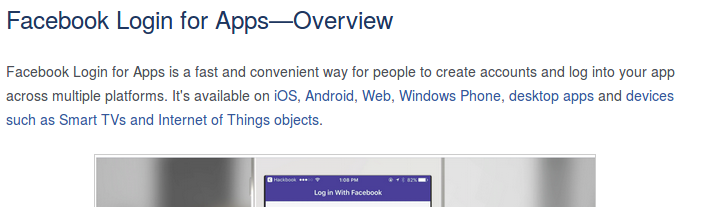
\includegraphics[width=0.7\textwidth]{fb-login-api}
\end{frame}

\begin{frame}[label=ssoLogin]{deliberate sharing: single-sign-on API}
\vspace{-.5cm}
    \begin{tikzpicture}
        \tikzset{
            >=Latex,
        }
        \node[fill=blue!30,minimum height=8cm,anchor=north west] (browser) at (0,0) { browser };
        \node[fill=green!30,minimum height=2cm,anchor=north east] (server1) at (15,0){ \tt example.com };
        \node[fill=yellow!30,minimum height=2cm,anchor=north east] (server2) at (15, -2.5) { \tt socialnetwork };
        \node[fill=green!30,minimum height=3cm,anchor=north east] (server3) at (15, -5) { \tt example.com};
        \begin{scope}[>=Latex,ultra thick,every node/.style={font=\tt\fontsize{10}{10}\selectfont,align=left,inner sep=.25mm},y=1.2cm]
            \draw[->] ([yshift=-.5cm]browser.north east) -- ([yshift=-.5cm]server1.north west)
                node[midway,above] { GET /login/ };
            \draw[<-] ([yshift=-1.5cm]browser.north east) -- ([yshift=-1.5cm]server1.north west)
                node[midway,above,align=center] (redirectOne) { Set-Cookie: ExSessionID=... \\ goto \texttt{socialnetwork/login/?for=example.com} };
            \draw[->] ([yshift=-3.0cm]browser.north east) -- ([yshift=-0.5cm]server2.north west)
                node[midway,above] { GET /login/?for=example.com \\ Cookie: SNSessionID=... };
            \draw[<-] ([yshift=-4.0cm]browser.north east) -- ([yshift=-1.5cm]server2.north west)
                node[midway,above] (redirectTwo) {  goto example.com/loggedin?\myemph{token=...} };
            \draw[->] ([yshift=-5.5cm]browser.north east) -- ([yshift=-0.5cm]server3.north west)
                node[midway,above] (token) { GET /loggedin?\myemph<2>{token=...} \\ Cookie: ExSessionID=... };
            \draw[<-] ([yshift=-6.5cm]browser.north east) -- ([yshift=-1.5cm]server3.north west)
                node[midway,above] { goto example.com/frontpage };
        \end{scope}
        \begin{visibleenv}<2>
            \node[my callout2=redirectOne,anchor=center,align=left] at ($(browser.east)!0.5!(server2.west)$) {
                tell browser to make request to socialnetwork; \\
                they will handle login
            };
        \end{visibleenv}
        \begin{visibleenv}<3>
            \node[my callout2=redirectTwo,anchor=center,align=left] at ([yshift=2cm]$(browser.east)!0.5!(server2.west)$) {
                socialnetwork verifies user's cookie \\
                (maybe displays login prompt) \\
                then redirects back to example.com with \myemph{token}
            };
        \end{visibleenv}
        \begin{visibleenv}<4>
            \node[my callout2=token,anchor=center,align=left] at ($(browser.east)!0.5!(server2.west)$) {
                example.com can \myemph{send token to socialnetwork to verify} \\
                e.g. make request to socialnetwork to get username 
            };
        \end{visibleenv}
    \end{tikzpicture}
\end{frame}

\begin{frame}{deliberate sharing: retrieving information}
    \begin{itemize}
    \item what about retrieving information from JavaScript?
    \item example: Google Translator API
    \item example: Token to Username API
    \vspace{.5cm}
    \item explicit mechanism for server opt-in to cross-origin requests (where webpage can read result)
        \begin{itemize}
        \item Cross-Origin Resource Sharing
        \end{itemize}
    \item \myemph{no opt-in? JS fails} like before
    \item always sends Origin --- no pretending to be innocent user
    \end{itemize}
\end{frame}

